\section{Auswertung}
\label{sec:Auswertung}

\subsection{Abweichung der Justierung}

Die in Schaltung 1 (siehe Abbildung \ref{fig:foto}) verbauten Kenngrößen sind sind in 
Tabelle \ref{tab:komponenten_schaltung1} zu sehen.
\begin{table}
    \centering
    \caption{Werte der in Schwingkreis 1 verbauten Komponenten}
    \label{tab:komponenten_schaltung1}
    \begin{tabular}{c c}
        \toprule
        Kompentente &  Wert \\
        \midrule
        L               & $23.954 \, \unit{\milli\henry}$   \\
        C               & $0.7932 \, \unit{\nano\farad}$    \\
        $C_{\text{Sp}}$ & $ 0.028 \, \unit{\nano\farad}$    \\
        R               & $ 48 \, \unit{\ohm}$              \\
        \bottomrule
    \end{tabular}
\end{table}

Wobei $C_{\text{Sp}}$ die Kapazität der realen Spule entspricht, wie der Abblildung 
\ref{fig:spulenkapazität} entnommen werden kann.
\begin{figure} 
    \centering
    \includegraphics[width=10cm] {pictures/spulenkapazität.png}  
    \caption{Berücksichtigung der Spulenkapazität $\text{C}_{\text{Sp}}$. \cite{v355}}
    \label{fig:spulenkapazität}
\end{figure} 

Die bei der Justierung gemessene Resonanzfrequenz des ersten Schwingkreises beträgt
\begin{equation*}
    \nu^+_{\text{gemessen}} = \qty{35.7}{\kilo\hertz} \, .
\end{equation*}

Mithilfe von (\ref{eq:resonanzfrequenzen}) lässt sich die theoretische Fundamentalfrequenz 
von Schwingkreis 1 errechnen:
\begin{equation}
    \nu^+ = \frac{1}{2 \pi} \cdot \frac{1}{\sqrt{L C}}= \qty{36.51}{\kilo\hertz}
    \quad \text {bzw.} \quad
    \nu^+ = \frac{1}{2 \pi} \cdot \frac{1}{\sqrt{L\left(C+C_{\mathrm{SP}}\right)}}= \qty{35.88}{\kilo\hertz} 
\end{equation}

Die Ergebnisse zwischen Messung und Theoriewerte stimmen mit geringer Abweichung
überein (siehe Tabelle \ref{tab:abweichung_schaltung1}).
\begin{table}
    \centering
    \caption{Werte der in Schwingkreis 1 verbauten Komponenten}
    \label{tab:abweichung_schaltung1}
    \begin{tabular}{c c}
        \toprule
        {Betrachtete Kapazität $\mathbin{/} \, \unit{\nano\farad}$} &
        {Abweichung $\mathbin{/} \, \unit{\percent}$} \\
        \midrule
        C = 0.7932                                   & 2.3  \\
        $\text{C} + \text{C}_{\text{Sp}} = 0.8212$   & 0.5  \\
        \bottomrule
    \end{tabular}
\end{table}


\subsection{Verhältnis Schwingung- und Schwebungsfrequenz}

Die Verhältnisse der Schwingungs- und Schwebungsfrequenz lassen sich anhand der
Anzahl an Schwingungen pro Schwebung bestimmen (siehe Tabelle \ref{tab:maxima}).
\begin{table} [H]
    \centering
    \caption{Anzahl der bei der Messung ersichtlichen Maxima/Minima der Schwebungen im Vergleich mit dem Theoriewert.}
    \label{tab:maxima}
    \begin{tabular}{c c c c}
        \toprule
        ${C_\text{K}} \mathbin{/} \unit{\nano\farad}$ &  Maxima &
        $n$ & $\increment n_{\text{rel}} \mathbin{/} \unit{\percent}$ \\
        \midrule
            2.19 &       4  &  3.69 &  7.69 \\
            2.86 &       5  &  4.55 &  9.01 \\
            4.74 &       7  &  6.94 &  0.90 \\
            6.86 &       9  &  9.62 &  6.85 \\
            8.18 &      10  & 11.28 & 12.82 \\
            9.99 &      11  & 13.56 & 23.31 \\
            12.00 &      12 & 16.10 & 34.14 \\
        \bottomrule
    \end{tabular}
\end{table}

Die Frequenzen werden in Tabelle \ref{tab:schwebung} mithilfe von (\ref{eq:resonanzfrequenzen}), 
(\ref{eq:schwebung}) und (\ref{eq:schwingung}) theoretisch berechnet. Der Koppelkondensator
$C_\text{K}$ besitzt dabei einen Fehler von 0.3 $\unit{\percent}$, der sich wie in Kapitel 
\ref{sec:Fehlerrechnung} beschrieben fortpflanzt.
\begin{table}
    \centering
    \caption{   Berechnung der Schwingungs- und Schwebungsfrequenz anhand der Theoriewerte
                in Abhängigkeit der Kapazität $C_\text{K}$. }
    \label{tab:schwebung}
    \begin{tabular}{c c c c c}
        \toprule
        ${C_\text{K}} \mathbin{/} \unit{\nano\farad}$ &
        $\nu^+_{t} \mathbin{/} \unit{\kilo\hertz}$ &
        $\nu^-_{t} \mathbin{/} \unit{\kilo\hertz}$ &
        $\nu_\text{Schwingung} \mathbin{/} \unit{\kilo\hertz}$ &
        $\nu_\text{Schwebung} \mathbin{/} \unit{\kilo\hertz}$ \\
        \midrule
         0.997${}\pm{}$0.003 &    36.51 & 58.77${}\pm{}$0.050 &    47.64${}\pm{}$0.027 &   22.26${}\pm{}$0.050 \\
          2.19${}\pm{}$0.007 &    36.51 & 47.95${}\pm{}$0.030 &    42.23${}\pm{}$0.015 &   11.44${}\pm{}$0.030 \\
          2.86${}\pm{}$0.009 &    36.51 & 45.53${}\pm{}$0.024 &    41.02${}\pm{}$0.012 &    9.02${}\pm{}$0.024 \\
          4.74${}\pm{}$0.014 &    36.51 & 42.18${}\pm{}$0.016 &    39.35${}\pm{}$0.008 &    5.67${}\pm{}$0.016 \\
          6.86${}\pm{}$0.021 &    36.51 & 40.51${}\pm{}$0.011 &    38.51${}\pm{}$0.006 &    4.00${}\pm{}$0.011 \\
          8.18${}\pm{}$0.025 &    36.51 & 39.90${}\pm{}$0.010 &    38.20${}\pm{}$0.005 &    3.39${}\pm{}$0.010 \\
          9.99${}\pm{}$0.030 &    36.51 & 39.30${}\pm{}$0.008 &    37.91${}\pm{}$0.004 &    2.79${}\pm{}$0.008 \\
         12.00${}\pm{}$0.040 &    36.51 & 38.85${}\pm{}$0.007 &    37.68${}\pm{}$0.003 &    2.34${}\pm{}$0.007 \\
        \bottomrule
    \end{tabular}
\end{table}

Die Größe $n$ in Tabelle \ref{tab:maxima} beschreibt das Verhältnis zwischen Schwingungs- und 
Schwebungsfrequenz. Somit gibt es die Anzahl der Maxima bzw. Minima innerhalb der Schwebung an. 
Die Maxima und Minima wechseln nach jeder $\pi$ Periode der Schwebung, sodass die Anzahl der Maxima
immer $\pi$ periodisch zwischen den zwei Werten schwankt. Die Berechnung von $n$ erfolgt dabei mit
\begin{equation}
    n=\frac{\nu^+ + \nu^-}{2\left(\nu^- - \nu^+\right)}=\frac{\nu_{\text{Schwingung}}}{\nu_{\text{Schwebung}}} \, .
\end{equation}

Zu beachten ist, dass die Messwerte
ganzzahlige Maxima darstellen, während die Theoriewerte das exakte Verhältnis von
Schwingungs- und Schwebungsfrequenz angeben. Die Berechnung der Abweichung $\increment n_{\text{rel}}$ erfolgt durch
\begin{equation}
    \increment n_{\text{rel}} = \frac{\increment n}{n}=\frac{\left|n-n_{t}\right|}{n} \, .
\end{equation}


\subsection{Die Frequenzen der Fundamentalschwingungen}

Die Ergebnisse der Messungen sind in Tabelle \ref{tab:vergleich} zu sehen, während die
theoretischen Frequenzen der Fundamentalschwingungen bereits bei der
Ermittelung der Verhältnisse zwischen Schwingungs- und Schwebungsfrequenz berechnet
wurden (siehe Tabelle \ref{tab:schwebung}). Der dabei auftretende Fehler wird in der Diskussion behandelt.
\begin{table}
    \centering
    \caption{   Vergleich der Theorie und Messwerte der Frequenzen der Fundamental-
                schwingungen. Die dabei genutzten Werte stammen aus Tabelle
                \ref{tab:maxima} und \ref{tab:schwebung}.}
    \label{tab:vergleich}
    \begin{tabular}{c c c c c}
    \toprule
    & \multicolumn{2}{c}{Theoriewerte} & \multicolumn{2}{c}{Messwerte} \\
    \cmidrule(lr){2-3}\cmidrule(lr){4-5}
    {${C_\text{K}} \mathbin{/} \unit{\nano\farad}$} &
    {$\nu^+_{t} \mathbin{/} \unit{\kilo\hertz}$} & {$\nu^-_{t} \mathbin{/} \unit{\kilo\hertz}$} &
    {$\nu^+ \mathbin{/} \unit{\kilo\hertz}$} & {$\nu^- \mathbin{/} \unit{\kilo\hertz}$} \\
    \midrule
    0.997${}\pm{}$0.003 &    36.51 & 58.77${}\pm{}$0.050 &    35.1 &   55.8 \\
     2.19${}\pm{}$0.007 &    36.51 & 47.95${}\pm{}$0.030 &    35.1 &   43.9 \\
     2.86${}\pm{}$0.009 &    36.51 & 45.53${}\pm{}$0.024 &    35.1 &   46.1 \\
     4.74${}\pm{}$0.014 &    36.51 & 42.18${}\pm{}$0.016 &    35.1 &   40.7 \\
     6.86${}\pm{}$0.021 &    36.51 & 40.51${}\pm{}$0.011 &    35.1 &   39.2 \\
     8.18${}\pm{}$0.025 &    36.51 & 39.90${}\pm{}$0.010 &    35.1 &   38.6 \\
     9.99${}\pm{}$0.030 &    36.51 & 39.30${}\pm{}$0.008 &    35.1 &   38.0 \\
    12.00${}\pm{}$0.040 &    36.51 & 38.85${}\pm{}$0.007 &    35.1 &   37.5 \\
    \bottomrule
    \end{tabular}
\end{table}

% Die Frequenz der Fundamentalschwingungen $\nu^-$ findet sich grafisch visualisiert in der
% Abbildung \ref{fig:plot1}.
\begin{figure}[H]
    \centering
    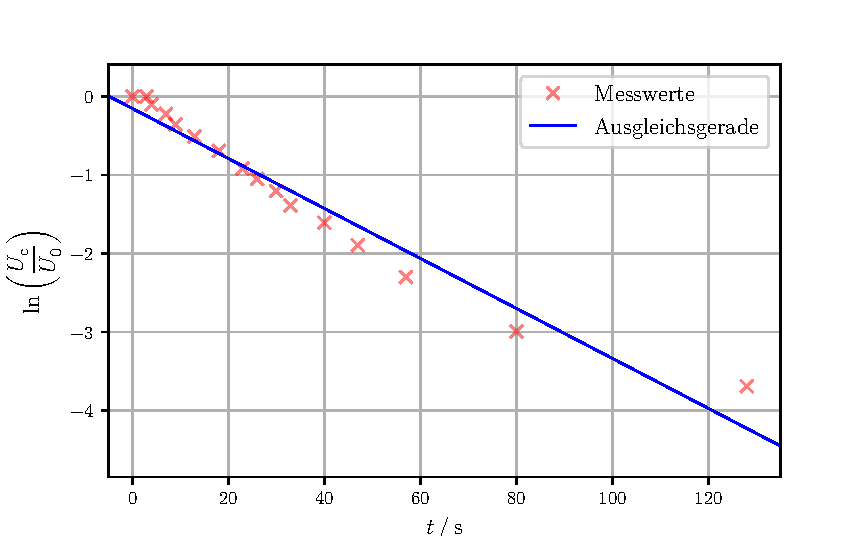
\includegraphics[width=0.75\textwidth]{plot1.pdf}
    \caption{Theorie- und Messwerte der Fundamentalschwingung $\nu^-$ in Abhängigkeit
    der Kapazität ${C_\text{K}}$.}
    \label{fig:plot1}
\end{figure}

\subsection{Frequenzabhängige Stromstärke}

Die Fundamentalfrequenzen sind die Frequenzen, für die der Strom, maximal wird. 
Daraus und dem \textit{ohmschen Gesetz} $U = R \cdot I$ folgt, dass auch die Sinusspannung maximal wird,
welche sich in Form von Amplitude. innerhalb des Frequenzintervalls äußern.\\
\\
Es sei angemerkt, dass bei dieser Messung aus technischen Gründen auf einen analogen Aufbau mit anderen Kenngrößen
zurückgegriffen wurde (siehe Tabelle \ref{tab:komponenten_schaltung2}). Die hierbei gemessene Resonanzfrequenz ist 
\begin{equation*}
    \nu^+_{\text{gemessen}} = \qty{30.66}{\kilo\hertz} \, .
\end{equation*}

\begin{table}
    \centering
    \caption{Werte der im analogen Aufbau verbauten Komponenten.}
    \label{tab:komponenten_schaltung2}
    \begin{tabular}{c c}
        \toprule
        Kompentente &  Wert \\
        \midrule
        L               & $32.351 \, \unit{\milli\henry}$   \\
        C               & $0.8015 \, \unit{\nano\farad}$    \\
        $C_{\text{Sp}}$ & $ 0.037 \, \unit{\nano\farad}$    \\
        R               & $ 48 \, \unit{\ohm}$              \\
        \bottomrule
    \end{tabular}
\end{table}

Die mithilfe des Wobbelgenerators gemessenen Zeitpunkte der Amplituden sind in Tabelle \ref{tab:amplituden} zu sehen.
\begin{table}[H]
    \centering
    \caption{}
    \label{tab:amplituden}
    \begin{tabular}{c c c c c}
        \toprule
        ${C_\text{K}} \mathbin{/} \unit{\nano\farad}$ &
        {Amplitude bei $t \mathbin{/} \unit{\milli\second}$} &
        $\nu^+_{t} \mathbin{/} \unit{\kilo\hertz}$ &
        $\increment n_{\text{rel}} \mathbin{/} \unit{\percent}$ &
        $\nu^-_{t} \mathbin{/} \unit{\kilo\hertz}$ \\
        \midrule
           1.11${}\pm{}$0.003 &      2.25 &    22.22 &  27.52 & 48.86${}\pm{}$0.040 \\
           2.03${}\pm{}$0.006 &      2.00 &    25.00 &  18.46 & 41.81${}\pm{}$0.028 \\
           3.00${}\pm{}$0.009 &      1.75 &    28.57 &   6.81 & 38.72${}\pm{}$0.020 \\
           4.00${}\pm{}$0.012 &      1.75 &    28.57 &   6.81 & 36.99${}\pm{}$0.016 \\
           5.02${}\pm{}$0.015 &      1.50 &    33.33 &   8.72 & 35.90${}\pm{}$0.013 \\
           6.47${}\pm{}$0.019 &      1.50 &    33.33 &   8.72 & 34.91${}\pm{}$0.010 \\
           8.00${}\pm{}$0.024 &      1.50 &    33.33 &   8.72 & 34.24${}\pm{}$0.009 \\
           9.99${}\pm{}$0.030 &      1.50 &    33.33 &   8.72 & 33.67${}\pm{}$0.007 \\
        \bottomrule
        \end{tabular}
\end{table}

Die theoretische Fundamentalfrequenz $\nu^+_{t}$ und der relative Abweichung $\increment \nu^+_{\text{rel}}$
von der gemessenen Resonanzfrequenz berrechnen sich dabei mithilfe von
\begin{equation*}
    \nu^+ = \frac {1} {t} 
    \quad\text{und}\quad 
    \increment \nu^+_{\text{rel}} = \frac{\increment \nu^+}{\nu^+}=\frac{\left|\nu^+-\nu^+_{t}\right|}{\nu^+} \, .
\end{equation*}
Wobei $\nu^-_{t}$ analog zum ursprünglichen Aufbau nach (\ref{eq:resonanzfrequenzen}) berechnet wird.